\section{Introduction}

%% Background
Wide-area streaming analytics are becoming pervasive, especially with the
emerging class of Internet of Things (IoT) applications.  Large cities such as
London and Beijing have deployed millions of cameras for surveillance and
traffic control~\cite{london.surveillance, skynet}. Buildings are increasingly
equipped with a wide variety of sensors to improve building energy use, occupant
comfort, reliability and
maintenance~\cite{krioukov2012building}. Geo-distributed infrastructure, such as
content delivery network (CDN) analyzes user requests from machine logs over the
globe~\cite{mukerjee2015practical}. These applications need to transport,
distill and analyze streams of data in real time.

While existing stream processing systems and specialized analytical engines,
such as Spark Streaming~\cite{zaharia2013discretized} and
VideoStorm~\cite{zhang2017live}, are capable of handling large streams of data,
they are designed to work inside a high-bandwidth network, such as a single data
center (DC). The bandwidth across the wide-area is significantly
limited~\cite{hsieh17gaia, vulimiri2015global}. Recent studies show that the
growth of the WAN bandwidth has been decelerating for many
years~\cite{global2016telegeography} while traffic demands grows at a staggering
rate~\cite{index2013zettabyte}.

Back-hauling all the data is not only impractical, but also inefficient. Recent
works on WAN-aware systems promote pushing computations towards the
edge~\cite{satyanarayanan2009case, rabkin2014aggregation, pu2015low}. However,
communications are not entirely avoidable for the following reasons: (i) some
analytics require joining or aggregating data from multiple geo-distributed
sites~\cite{pu2015low, viswanathan2016clarinet}; (ii) the edge benefits
significantly from central computing resources such as GPU or
TPU~\cite{abadi2016tensorflow} in the cloud; (iii) end-devices such as cameras or
mobile devices suffer from the bandwidth in last-hop wireless
links~\cite{zhang2015design, abari2017enabling}.

% could improve efficiency (such as GDA pushes queries out; cloudlet
% etc). However, we still need data transmission for cloud off-loading or
% aggregation purpose.

When facing insufficient bandwidth, application developers need to make a
decision within the design space of data freshness and data fidelity
(\autoref{fig:intro}):

\begin{figure}
  \centering
  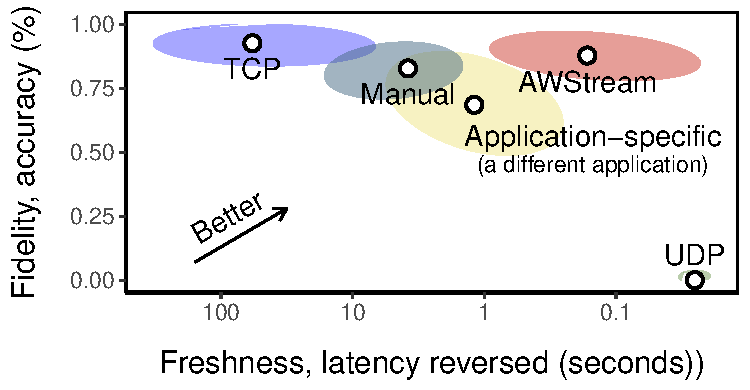
\includegraphics[width=0.9\columnwidth]{figures/figure1a.pdf}
  \caption{The trade-off space between data freshness and data fidelity when
    facing insufficient bandwidth.}
  \label{fig:intro}
  \vspace{-1em}
\end{figure}

Widely-used protocols often work at one extreme point in the design space. TCP
ensures a reliable data delivery but the backlogged data increases application
latency. UDP minimizes the latency by sending packets as fast as possible, but
uncontrolled packet loss devastates application behavior.

Manual policies, such as sampling~\cite{rabkin2014aggregation}, allows
developers to trade data fidelity for freshness. But it's non-trivial to write
accurate policies. In practice, these policies are developer heuristics without
measurements backing up, leading to sub-optimal performance for both freshness
and fidelity.

Application-specific optimizations do not generalize. While developers may tune
policies or algorithms for a specific application, these solutions will work
poorly when the application goal or data distribution changes. Video streaming,
for example, has primarily focused on improving quality of experience
(QoE)~\cite{yin2015control}. Because humans favor smoothness over image quality,
video streaming maintains a high frame rate, e.g. 25FPS. Such a restriction is
unnecessary for machine-based video processing.

To address the bandwidth limitations from a system level, we propose to augment
existing stream processing models with \textit{structured
  adaptation~(SA)}. Instead of developers writing manual policies or tuning
individual applications, SA defines a set of operators that tolerate approximate
specifications, and synthesizes an accurate policy (profile) automatically. In
this paper, we present the design and evaluation of \sysname{} that implements
SA.

Along with with normal stream processing operators, \sysname{} has a new
\maybe{} operator, whose basic form takes a list of values as a knob and a
function that degrades the input stream. We extend the basic form with a library
of specialized operators for common data types, such as
\texttt{maybe\_downsample} for images.  Our APIs are simple, modular and
extensible. Developers do not need to be an expert in the application domain as
the knobs tolerate approximate specifications. Multiple operators can be chained
to form a configuration that affects the adaptation jointly. Arbitrary functions
including external libraries can be embedded with our operators.

\sysname{} then uses a data-driven approach to automatically build application
performance profiles with minimal developer effort. The profiles accurately
capture the relationship between application accuracy and bandwidth consumption
under different combinations of data degradation operations. We use an offline
process to bootstrap our system with developer-supplied training data, and
continuously refine the profiles online to handle potential model drifts. We
exploit parallelism and partial profiling to efficiently explore the
configuration space and learn a Pareto-optimal adaptation strategy.

At runtime, \sysname{} achieves low latency by matching data rate to available
bandwidth, and high accuracy by using the Pareto-optimal configuration from the
profile. Upon network congesting, our rate adaptation algorithm increases the
degradation level such that no persistent queue builds up. To recover, it probes
for more bandwidth in a fine-grain manner and decreases the degradation level
progressively. The runtime can control application behaviors based on the
profile in other ways. For instance, developers can limit the maximum allowed
bandwidth to reduce WAN cost or allocate bandwidth among competing tasks for
utility-fairness, i.e. maximizing the minimal accuracy.

To evaluate \sysname{}, we've built three streaming applications: pedestrian
detection (PD), augmented reality (AR) and a distributed Top-K (TK). We use
real-world data to profile these applications and evaluate their runtime
performance with controlled experiments using geo-distributed
infrastructure. Our contributions and evaluation results are summarized as
follows:

\begin{itemize}[leftmargin=16pt]

\item We propose to incorporate structured adaptation as a first-class citizen
  in the stream processing model. Such a programming abstraction is simple,
  modular and extensible. We implement SA in \sysname{} and evaluate the idea
  with three real-world applications.

\item Our profiler learns an accurate and precise profile for each
  application. We show that parallelism and partial profiling can speed up the
  profiling substantially, up to 29X and 8X respectively.

\item Our runtime achieves low latency and high accuracy simultaneously for all
  applications: sub-second latency and 5\% accuracy drop for video analytics,
  4-second latency and 6\% accuracy drop for TK.

\end{itemize}

%%% Local Variables:
%%% mode: latex
%%% TeX-master: "sosp17"
%%% End:

%% LocalWords: VideoStorm, analytics, CDN, IoT
